\chapter{直流-直流変換(1) 非絶縁型}
\label{chap5}

いよいよ変換回路の各論に入る。第I部で手に入れた半導体スイッチと，4章のインダクタ・キャパシタを組み合わせ，
直流電圧を別の直流電圧に作り替える\index{でぃーしーでぃーしーへんかん@DC-DC変換}\textbf{DC-DC変換}を扱う。
本章の3つの回路（降圧・昇圧・昇降圧チョッパ）は部品数こそ少ないが，
スイッチング電源の考え方のすべてが詰まっており，6章以降のどの変換回路も本章の考え方の組合せで読める。その意味で本章は本書全体の要の章である。

\begin{screen}
\noindent\textbf{本章の現在地}\\[3pt]
序章の電力変換の地図（\ref{fig0.1}）の「直流→直流」に入る（5〜7章）。
本章はその第1歩，トランスを使わない\index{ひぜつえんがた@非絶縁型}\textbf{非絶縁型}のチョッパ回路である。
エネルギーの視点で先に要点を言えば，\textbf{オン期間にインダクタへ蓄え，オフ期間に放出する ―
蓄えと放出の比率がそのまま電圧比になる}。本章の式はすべてこの1行の言い換えである。
\end{screen}

%%======================================================================
\section{DC-DC変換とは}
\label{sec5.1}

\subsection{直流電圧を作り替える3つの方法}

直流5\,Vで動くマイコンも，48\,Vのバッテリーで動くモータも，もとをたどれば別の電圧の直流から給電されていることが多い。
直流電圧を目的の値に作り替える方法は，大きく次の3つに分けられる。

\begin{箇条書}
\item \textbf{非絶縁型チョッパ回路}：スイッチングによる変換。本章で扱う
\item \textbf{絶縁型コンバータ}：トランスを介して絶縁しながら変換する（6章）
\item \textbf{リニアレギュレータ}：余分な電圧を抵抗として連続的に落とす（7章）
\end{箇条書}

\index{ちょっぱ@チョッパ}\textbf{チョッパ}（chopper）とは「刻むもの」の意味で，半導体スイッチで入力電圧を高速に刻み，その平均値を制御する回路である。
理想的にはスイッチは「電圧ゼロで電流を流す」か「電流ゼロで電圧を受け持つ」かのどちらかの状態しか取らないため，原理的に損失がない。
効率よく，かつ小さな部品で大きな電力を扱えることがチョッパ方式の利点であり，現代の電源回路の主流である。

スイッチングの時間配分を表すのが次のデューティ比である。

\begin{定義}[デューティ比]
\label{def5.1}
スイッチを周期$T$（\index{すいっちんぐしゅうき@スイッチング周期}スイッチング周期）でオン・オフし，そのうちオンの時間を$T_{\mathrm{on}}$とするとき，
\begin{equation}
D = \frac{T_{\mathrm{on}}}{T}
\label{eq5.1}
\end{equation}
を\index{でゅーてぃひ@デューティ比}\textbf{デューティ比}という（$0 < D < 1$）。
$f = 1/T$を\index{すいっちんぐしゅうはすう@スイッチング周波数}\textbf{スイッチング周波数}という。
\end{定義}

本章の主役はこの$D$である。後で示すように，3つのチョッパ回路の出力電圧はいずれも$D$だけで決まり，$D$を変えることで出力を連続的に制御できる。

\subsection{定常状態とボルト秒平衡 ― 4章の引き継ぎ}

チョッパ回路の解析の鍵は，4章で学んだインダクタの性質である。インダクタの電圧$v_L$と電流$i_L$の関係
\begin{equation}
v_L = L \frac{d i_L}{d t}
\label{eq5.2}
\end{equation}
を$0$から$T$まで積分すると，1周期の間の電流の変化が求められる。
\begin{equation}
i_L(T) - i_L(0) = \frac{1}{L} \int_0^T v_L(t)\, dt
\label{eq5.3}
\end{equation}
回路に電源を入れた直後は，この値は正で，電流は周期ごとに増えていく（過渡状態）。
やがて毎周期同じ波形を繰り返す\index{ていじょうじょうたい@定常状態}\textbf{定常状態}に落ち着くと，
$i_L(T) = i_L(0)$，すなわち1周期あたりの電流の増減はゼロになる。このとき式\ref{eq5.3}の右辺の積分もゼロでなければならない。

\begin{定理}[ボルト秒平衡]
\label{th5.1}
定常状態では，インダクタ電圧の1周期の積分はゼロになる。
\begin{equation}
\int_0^T v_L(t)\, dt = 0
\label{eq5.4}
\end{equation}
すなわち，インダクタ電圧の波形の正の面積と負の面積（ボルト$\times$秒）は等しい。
\end{定理}

これを\index{ぼるとびょうへいこう@ボルト秒平衡}\textbf{ボルト秒平衡}という。エネルギーの言葉で言えば，
オン期間に磁場として蓄えたエネルギーを，オフ期間にちょうど使い切る（蓄えっぱなしでも足りなくもならない）状態が定常状態である。

本章の回路では，$v_L$はオン期間とオフ期間でそれぞれ一定値$V_{\mathrm{on}}$，$V_{\mathrm{off}}$を取る。このとき式\ref{eq5.4}の積分は長方形の面積の和になるから，
\begin{equation}
V_{\mathrm{on}} \cdot DT + V_{\mathrm{off}} \cdot (1-D)T = 0
\label{eq5.5}
\end{equation}
と書ける。$V_{\mathrm{on}}$と$V_{\mathrm{off}}$は回路ごとにキルヒホッフの電圧則から求まるので，
式\ref{eq5.5}に代入すれば出力電圧が得られる。以降の3つの回路はすべて，この同じ手順で解析する。

\begin{screen}
\noindent\textbf{手順：チョッパ回路の解析}\\[3pt]
\begin{enumerate}
\item 仮定を明示する（理想素子・定常状態・電流連続・リプル小）
\item オン期間とオフ期間の\index{とうかかいろ@等価回路}\textbf{等価回路}を描く
\item 各期間の$v_L$を求め，ボルト秒平衡（式\ref{eq5.5}）に代入して電圧比を得る
\item 波形を描き，エネルギーの流れを言葉で確かめる
\end{enumerate}
\end{screen}

\begin{問}
\item スイッチング周波数$f = 100$\,kHzで，デューティ比$D = 0.3$とする。
スイッチング周期$T$とオン時間$T_{\mathrm{on}}$を求めよ。また，$0$\,Vと$12$\,Vを行き来するこのスイッチング波形の平均電圧を求めよ。
\end{問}

%%======================================================================
\section{降圧チョッパ}
\label{sec5.2}

\subsection{回路構成}

\index{こうあつちょっぱ@降圧チョッパ}\textbf{降圧チョッパ}（\index{ばっくこんばーた@バックコンバータ}バックコンバータ，buck converter）は，
入力電圧$V_{\mathrm{in}}$より低い出力電圧$V_{\mathrm{out}}$を作る回路である（\FIGref{fig5.1}(a)）。登場する素子は4つで，役割がはっきり分かれている。

\begin{箇条書}
\item スイッチS：入力電圧を刻む（MOSFETなど。2章）
\item ダイオード$\mathrm{D}$：Sがオフの間，インダクタ電流の通り道を作る。この役割のダイオードを\index{かんりゅうだいおーど@還流ダイオード}\textbf{還流ダイオード}
（\index{ふりーほいーるだいおーど@フリーホイールダイオード}フリーホイールダイオード）という
\item インダクタ$L$：電流を平滑にし，エネルギーを蓄えて受け渡す
\item キャパシタ$C$：出力電圧を平滑にする（\index{へいかつきゃぱした@平滑キャパシタ}\textbf{平滑キャパシタ}）
\end{箇条書}

\begin{figure}[ht]
\begin{center}
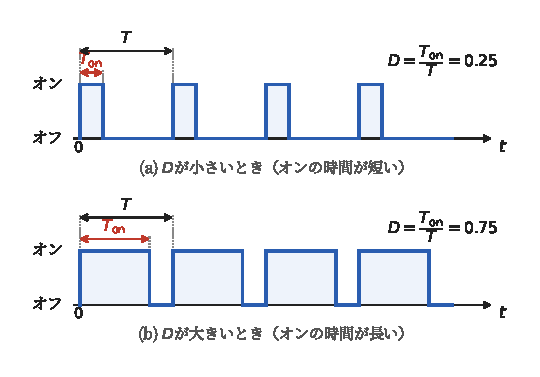
\includegraphics[clip]{figures/fig5.1.eps}
\end{center}
\caption{降圧チョッパ。(a)回路構成，(b)オン期間，(c)オフ期間の等価回路。灰色は電流が流れない部分，赤の矢印は電流の経路を表す}
\label{fig5.1}
\end{figure}

解析に入る前に，置いている仮定をはっきりさせておく。

\begin{注意}
本章の解析では次の4つを仮定する。(1)~スイッチとダイオードは理想的（オンで電圧降下ゼロ，オフで電流ゼロ，切替えは一瞬）。
(2)~回路は定常状態にある。(3)~インダクタ電流は常に正である
（\index{でんりゅうれんぞくもーど@電流連続モード}\textbf{電流連続モード}。\ref{sec5.7}節で崩れる場合を扱う）。
(4)~出力電圧のリプルは小さく，$v_{\mathrm{out}}$は一定値$V_{\mathrm{out}}$とみなせる。仮定が崩れるとどうなるかは\ref{sec5.7}節と章末問題\ref{ex5.5}で確かめる。
\end{注意}

\subsection{オン期間とオフ期間の等価回路}

\textbf{オン期間}（$0 \le t < DT$）は，Sが導通し，電流は電源→S→$L$→負荷の経路を流れる（\ref{fig5.1}(b)）。
このときダイオードには$V_{\mathrm{in}}$が逆向きにかかるので導通しない（切り離されたのと同じ）。
経路に沿ってキルヒホッフの電圧則を立てると$V_{\mathrm{in}} = v_L + V_{\mathrm{out}}$，すなわち
\begin{equation}
v_L = V_{\mathrm{in}} - V_{\mathrm{out}}
\label{eq5.6}
\end{equation}
である。降圧チョッパでは$V_{\mathrm{in}} > V_{\mathrm{out}}$だから$v_L > 0$，
式\ref{eq5.2}より電流$i_L$は一定の傾き$(V_{\mathrm{in}}-V_{\mathrm{out}})/L$で増える。インダクタは磁場にエネルギーを蓄えていく。

\textbf{オフ期間}（$DT \le t < T$）は，Sが切れる。しかし4章で見たとおり，インダクタは電流を続けようとする。
行き場を失った電流はダイオードを押し開け，$\mathrm{D}$→$L$→負荷の経路で流れ続ける（\ref{fig5.1}(c)）。
ダイオードの電圧降下をゼロとすると，$L$と負荷のループについて$0 = v_L + V_{\mathrm{out}}$，すなわち
\begin{equation}
v_L = -V_{\mathrm{out}}
\label{eq5.7}
\end{equation}
である。$v_L < 0$だから電流は傾き$-V_{\mathrm{out}}/L$で減り，蓄えたエネルギーが負荷へ放出される。

\subsection{ボルト秒平衡から電圧比を導く}

式\ref{eq5.6}と式\ref{eq5.7}をボルト秒平衡（式\ref{eq5.5}）に代入する。
\begin{equation}
(V_{\mathrm{in}} - V_{\mathrm{out}}) \cdot DT+ (-V_{\mathrm{out}}) \cdot (1-D)T = 0
\label{eq5.8}
\end{equation}
両辺を$T$で割って展開すると
\begin{eqnarray}
V_{\mathrm{in}} D - V_{\mathrm{out}} D - V_{\mathrm{out}} + V_{\mathrm{out}} D &=& 0 \nonumber\\
V_{\mathrm{in}} D - V_{\mathrm{out}} &=& 0 \nonumber
\end{eqnarray}
となり，出力電圧が得られる。
\begin{equation}
V_{\mathrm{out}} = D\, V_{\mathrm{in}}
\label{eq5.9}
\end{equation}
$0 < D < 1$だから，出力は必ず入力より低い。そして$D$を変えれば$0$から$V_{\mathrm{in}}$まで連続的に制御できる。
「オン期間の割合＝電圧の比」という最も素直な変換である。

\begin{figure}[ht]
\begin{center}
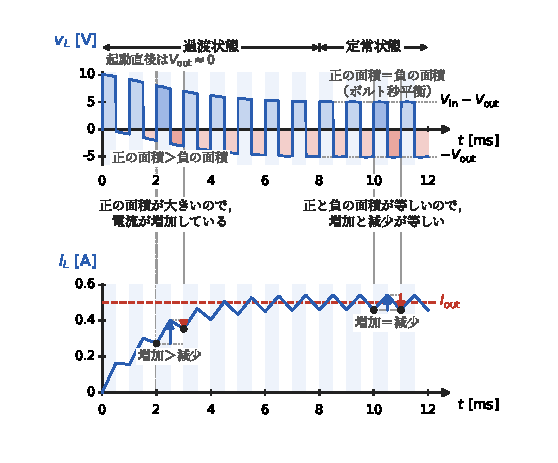
\includegraphics[clip]{figures/fig5.2.eps}
\end{center}
\caption{降圧チョッパの定常状態波形。$v_L$の正負の面積が等しく（ボルト秒平衡），
$i_L$は三角波状に増減する。$i_L$の変動分はキャパシタ電流$i_C$となり，平均値$I_{\mathrm{out}}$だけが負荷へ流れる}
\label{fig5.2}
\end{figure}

定常状態の波形を\FIGref{fig5.2}に示す。$v_L$は$V_{\mathrm{in}}-V_{\mathrm{out}}$と$-V_{\mathrm{out}}$の2値の矩形波，
$i_L$は平均値$I_{\mathrm{out}}$のまわりを直線的に増減する三角波である。この三角波の振れ幅（\ref{sec5.5}節のリプル電流）と，
それをキャパシタが受け持つことで生じる出力電圧の振れ（\ref{sec5.6}節）が，そのまま$L$と$C$の設計につながる。

\textbf{エネルギーの流れ}：オン期間は電源が負荷へ電力を送りながら，余り分を$L$の磁場に蓄える。
オフ期間は電源が切り離され，$L$が蓄えを放出して負荷への供給を続ける。負荷から見れば途切れなく電力が届く ―
インダクタが「電源が休んでいる間の中継ぎ」を務めるのである。

\begin{例題}[降圧チョッパの動作点]
\label{rei5.1}
入力$12$\,Vの降圧チョッパで出力$5$\,Vを得たい。スイッチング周波数を$f = 100$\,kHzとするとき，
デューティ比$D$と，1周期のうちSおよび$\mathrm{D}$が導通する時間を求めよ。
\begin{解答}
式\ref{eq5.9}より
\begin{equation*}
D = \frac{V_{\mathrm{out}}}{V_{\mathrm{in}}} = \frac{5}{12} \approx 0.417
\end{equation*}
周期は$T = 1/f = 10\,\mathrm{\mu s}$だから，Sの導通時間は$DT \approx 4.2\,\mathrm{\mu s}$，
ダイオードの導通時間は$(1-D)T \approx 5.8\,\mathrm{\mu s}$である。この動作点は\ref{sec5.5}節・\ref{sec5.6}節の設計例題でも使う。
\end{解答}
\end{例題}

\begin{問}
\item 入力$48$\,Vから出力$12$\,Vを作る降圧チョッパのデューティ比を求めよ。また，オフ期間にスイッチSの両端にかかる電圧を求めよ。
\end{問}

%%======================================================================
\section{昇圧チョッパ}
\label{sec5.3}

\subsection{どうすれば入力より高い電圧が作れるか}

抵抗で分圧しても，スイッチで刻んで平均しても，入力より高い電圧は作れない。入力より高い電圧を作るには，
\textbf{いったんエネルギーを蓄え，電源に上乗せして送り出す}しかない。これを実現するのが\index{しょうあつちょっぱ@昇圧チョッパ}\textbf{昇圧チョッパ}
（\index{ぶーすとこんばーた@ブーストコンバータ}ブーストコンバータ，boost converter）である（\FIGref{fig5.3}(a)）。素子は降圧チョッパと同じ4つだが，配置が違う。
インダクタが入力側に移り，スイッチSはインダクタの後で線路を接地側へ短絡する位置に，ダイオードは出力への一方通行弁の位置に置かれる。
仮定は\ref{sec5.2}節の注意と同じである（理想素子・定常状態・電流連続・リプル小）。

\begin{figure}[ht]
\begin{center}
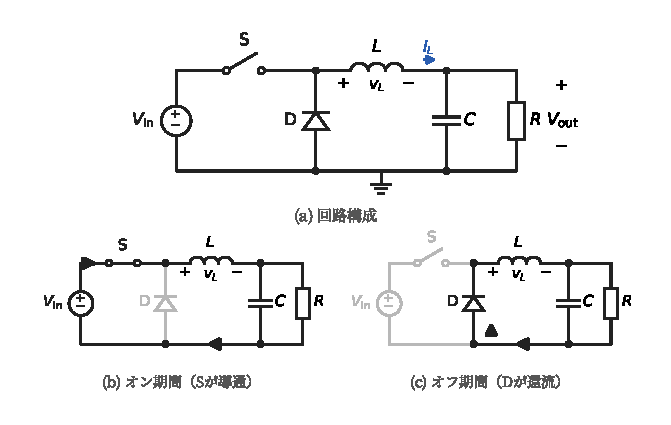
\includegraphics[clip]{figures/fig5.3.eps}
\end{center}
\caption{昇圧チョッパ。(a)回路構成，(b)オン期間，(c)オフ期間の等価回路。オン期間は出力がダイオードで切り離され，$C$が負荷への供給を受け持つ}
\label{fig5.3}
\end{figure}

\subsection{オン期間とオフ期間の等価回路}

\textbf{オン期間}（$0 \le t < DT$）は，Sが導通して電源→$L$→Sのループができる（\ref{fig5.3}(b)）。このループのキルヒホッフの電圧則は$V_{\mathrm{in}} = v_L$，すなわち
\begin{equation}
v_L = V_{\mathrm{in}}
\label{eq5.10}
\end{equation}
である。入力電圧のすべてがインダクタにかかり，電流は傾き$V_{\mathrm{in}}/L$で増えて，エネルギーが磁場に蓄えられる。
このとき出力側では，ダイオードに$V_{\mathrm{out}}$が逆向きにかかって遮断され（Sの導通で$\mathrm{D}$のアノードは接地電位，カソードは$V_{\mathrm{out}}$になる），
負荷への供給は平滑キャパシタ$C$の放電だけが受け持つ。

\textbf{オフ期間}（$DT \le t < T$）は，Sが切れる。電流を続けようとするインダクタが$\mathrm{D}$を押し開け，
電源→$L$→$\mathrm{D}$→負荷の経路ができる（\ref{fig5.3}(c)）。キルヒホッフの電圧則は$V_{\mathrm{in}} = v_L + V_{\mathrm{out}}$，すなわち
\begin{equation}
v_L = V_{\mathrm{in}} - V_{\mathrm{out}}
\label{eq5.11}
\end{equation}
である。昇圧チョッパでは$V_{\mathrm{out}} > V_{\mathrm{in}}$になる（すぐ後で示す）から$v_L < 0$，
電流は減りながら，\textbf{電源とインダクタが直列になって}負荷へエネルギーを送り込む。インダクタの電圧が電源に上乗せされる ― これが昇圧の正体である。

\subsection{ボルト秒平衡から電圧比を導く}

式\ref{eq5.10}と式\ref{eq5.11}をボルト秒平衡（式\ref{eq5.5}）に代入する。
\begin{equation}
V_{\mathrm{in}} \cdot DT + (V_{\mathrm{in}} - V_{\mathrm{out}}) \cdot (1-D)T = 0
\label{eq5.12}
\end{equation}
両辺を$T$で割って展開すると
\begin{eqnarray}
V_{\mathrm{in}} D + V_{\mathrm{in}} - V_{\mathrm{in}} D
- V_{\mathrm{out}} (1-D) &=& 0 \nonumber\\
V_{\mathrm{in}} - V_{\mathrm{out}} (1-D) &=& 0 \nonumber
\end{eqnarray}
となり，出力電圧が得られる。
\begin{equation}
V_{\mathrm{out}} = \frac{V_{\mathrm{in}}}{1-D}
\label{eq5.13}
\end{equation}
$0 < D < 1$だから$1-D < 1$，出力は必ず入力より高い。たとえば$D = 0.5$で2倍，$D = 0.8$で5倍になる。

\begin{figure}[ht]
\begin{center}
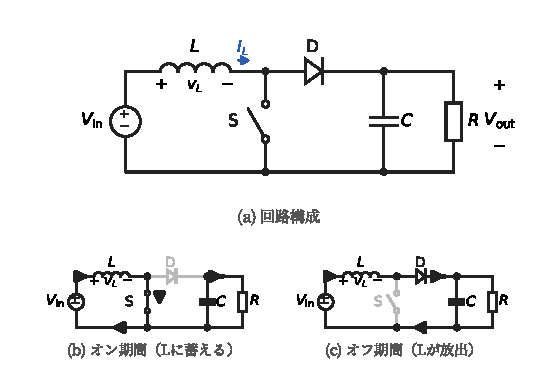
\includegraphics[clip]{figures/fig5.4.eps}
\end{center}
\caption{昇圧チョッパの定常状態波形。インダクタ電流$i_L$の平均は入力電流
$I_{\mathrm{in}}$であり，オフ期間だけダイオード電流$i_{\mathrm{D}}$として出力へ流れる。その平均が負荷電流$I_{\mathrm{out}}$になる}
\label{fig5.4}
\end{figure}

定常状態の波形を\FIGref{fig5.4}に示す。降圧チョッパと違い，$i_L$の平均は\textbf{入力電流}$I_{\mathrm{in}}$である。
出力へは，オフ期間だけダイオードを通して電流が届く。損失がなければ入力と出力の電力は等しいから
$V_{\mathrm{in}} I_{\mathrm{in}} = V_{\mathrm{out}} I_{\mathrm{out}}$であり，式\ref{eq5.13}を使うと
\begin{equation}
I_{\mathrm{in}} = \frac{V_{\mathrm{out}}}{V_{\mathrm{in}}}\, I_{\mathrm{out}}= \frac{I_{\mathrm{out}}}{1-D}
\label{eq5.14}
\end{equation}
となる。電圧を上げた分だけ，入力側には大きな電流が流れる。

\begin{注意}
式\ref{eq5.13}の上では$D \to 1$で出力は限りなく大きくなるが，実際にはそうならない。
$D$が1に近づくとオフ期間がごく短くなり，蓄えたエネルギーを送り出す時間が足りなくなる一方，
式\ref{eq5.14}のとおり入力電流が増大して，インダクタの巻線抵抗やスイッチのオン抵抗（3章）での損失が急増するからである。
実用的な昇圧比はせいぜい数倍までであり，それ以上はトランスを使う絶縁型（6章）の出番になる。
\end{注意}

\textbf{エネルギーの流れ}：オン期間は電源のエネルギーをすべて$L$に蓄え込み（その間の負荷は$C$が支える），
オフ期間に電源と$L$が力を合わせて，高い電圧で$C$と負荷へ送り出す。
「低い電圧で時間をかけて蓄え，高い電圧で短時間に放出する」― 蓄えと放出の時間配分が電圧比$1/(1-D)$を作っている。

\begin{例題}[昇圧チョッパの動作点]
\label{rei5.2}
バッテリー電圧$5$\,Vから$12$\,Vを作る昇圧チョッパについて，(a)~デューティ比$D$，(b)~出力電流が$0.42$\,Aのときの入力電流を求めよ。損失はないものとする。
\begin{解答}
(a) 式\ref{eq5.13}を$D$について解くと
\begin{equation*}
D = 1 - \frac{V_{\mathrm{in}}}{V_{\mathrm{out}}} = 1 - \frac{5}{12}= \frac{7}{12} \approx 0.583
\end{equation*}
(b) 式\ref{eq5.14}より
\begin{equation*}
I_{\mathrm{in}} = \frac{I_{\mathrm{out}}}{1-D}= \frac{0.42}{5/12} \approx 1.0\,\mathrm{A}
\end{equation*}
出力の2.4倍の電流が入力側に流れる。昇圧チョッパの入力側の配線・インダクタ・スイッチは，この大きな電流を前提に選ばなければならない。
\end{解答}
\end{例題}

\begin{問}
\item 太陽電池の$24$\,Vを$96$\,Vに昇圧したい。デューティ比を求めよ。また$D = 0.9$まで使えるとすると，理論上の最大出力電圧は入力の何倍か。
\end{問}

%%======================================================================
\section{昇降圧チョッパ}
\label{sec5.4}

\subsection{回路構成と動作}

入力より高い電圧も低い電圧も1つの回路で作れるのが\index{しょうこうあつちょっぱ@昇降圧チョッパ}\textbf{昇降圧チョッパ}
（\index{ばっくぶーすとこんばーた@バックブーストコンバータ}バックブーストコンバータ，buck-boost converter）である（\FIGref{fig5.5}(a)）。素子はやはり同じ4つで，
スイッチSが入力側，インダクタ$L$が中央で接地へ落ち，ダイオード$\mathrm{D}$が出力側を向く。仮定はこれまでと同じである。

\begin{figure}[ht]
\begin{center}
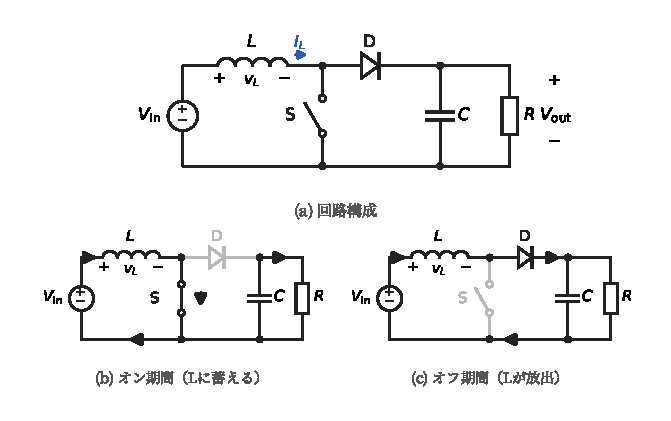
\includegraphics[clip]{figures/fig5.5.eps}
\end{center}
\caption{昇降圧チョッパ。(a)回路構成，(b)オン期間，(c)オフ期間の等価回路。
エネルギーはいったんすべて$L$に蓄えられてから負荷へ渡り，出力の極性が反転する（上の端子が負になる）}
\label{fig5.5}
\end{figure}

\textbf{オン期間}（$0 \le t < DT$）は，Sが導通して電源→S→$L$のループができ（\ref{fig5.5}(b)），
\begin{equation}
v_L = V_{\mathrm{in}}
\label{eq5.15}
\end{equation}
となる。昇圧チョッパのオン期間と同じく，入力のエネルギーはすべて$L$の磁場に蓄えられ，負荷は$C$が支える。このときダイオードは逆バイアスされて遮断されている。

\textbf{オフ期間}（$DT \le t < T$）は，Sが切れ，電流を続けようとする$L$が$\mathrm{D}$を押し開けて，$L$→負荷→$\mathrm{D}$のループができる（\ref{fig5.5}(c)）。
出力電圧$V_{\mathrm{out}}$を，これまでと同じ向き（図の上の端子を正）で測ると，理想ダイオードを介して$L$と負荷が並列につながるから
\begin{equation}
v_L = V_{\mathrm{out}}
\label{eq5.16}
\end{equation}
である。

\subsection{ボルト秒平衡から電圧比を導く}

式\ref{eq5.15}と式\ref{eq5.16}をボルト秒平衡（式\ref{eq5.5}）に代入する。
\begin{equation}
V_{\mathrm{in}} \cdot DT + V_{\mathrm{out}} \cdot (1-D)T = 0
\label{eq5.17}
\end{equation}
両辺を$T$で割って$V_{\mathrm{out}}$について解くと
\begin{equation}
V_{\mathrm{out}} = -\frac{D}{1-D}\, V_{\mathrm{in}}
\label{eq5.18}
\end{equation}
となる。大きさ$|V_{\mathrm{out}}|$は，$D < 0.5$で入力より低く（降圧），$D = 0.5$で等しく，$D > 0.5$で高くなる（昇圧）。1つの回路で両方向をカバーできる。

\begin{注意}
式\ref{eq5.18}の負号は，出力の\index{きょくせいはんてん@極性反転}\textbf{極性が反転}することを表す
（\ref{fig5.5}(a)の極性表示）。オン期間に$L$には上から下へ電流が流れ込み，オフ期間もインダクタはこの向きの電流を続けようとする。
その電流は負荷を\textbf{下から上へ}貫くから，出力の上の端子が負になるのである。
負電源を作れる利点でもあるが，制御回路の基準電位（グラウンド）の扱いには注意を要する。
\end{注意}

\textbf{エネルギーの流れ}：降圧チョッパではオン期間に電源から負荷へ直接電力が流れ，
昇圧チョッパではオフ期間に電源が直接負荷へ送り込んでいた。これに対して昇降圧チョッパでは，\textbf{エネルギーはいったんすべて$L$に蓄えられ，それから負荷へ渡される}。
電源と負荷が直接つながる瞬間がないから，蓄えの時間$DT$と放出の時間$(1-D)T$の配分しだいで，
電圧を低くも高くも作り替えられる。この「エネルギーをいったん磁場に預けて受け渡す」考え方は，
インダクタをトランスに置き換えた絶縁型コンバータ（6章）へそのままつながる。

3つのチョッパ回路の性質を\TABref{tab5.1}にまとめる。

\begin{table}[ht]
\begin{center}
\caption{3つのチョッパ回路の比較}
\label{tab5.1}
\begin{tabular}{c|c|c|c}
\hline
回路 & 電圧比$V_{\mathrm{out}}/V_{\mathrm{in}}$ & 出力範囲 & 極性 \\
\hline
降圧チョッパ & $D$ & $0 \sim V_{\mathrm{in}}$ & 入力と同じ \\
昇圧チョッパ & $\dfrac{1}{1-D}$ & $V_{\mathrm{in}}$以上 & 入力と同じ \\
昇降圧チョッパ & $-\dfrac{D}{1-D}$ & 0から昇圧域まで & 反転 \\
\hline
\end{tabular}
\end{center}
\end{table}

\begin{問}
\item 入力$12$\,Vの昇降圧チョッパで出力$-5$\,Vおよび$-24$\,Vを得るためのデューティ比をそれぞれ求めよ。
\end{問}

%%======================================================================
\section{リプル電流とインダクタの設計}
\label{sec5.5}

\subsection{リプル電流はオン期間の電流の増え幅}

ここからは設計の話に入る。\ref{fig5.2}で見たとおり，インダクタ電流は平均値のまわりを三角波状に増減する。
この振れの全幅（山から谷まで）を\index{りぷるでんりゅう@リプル電流}\textbf{リプル電流}$\mathit{\Delta}I_L$という。

$\mathit{\Delta}I_L$は波形を描くまでもなく計算できる。降圧チョッパのオン期間，電流は一定の傾き
$(V_{\mathrm{in}}-V_{\mathrm{out}})/L$で$DT$の間増え続けるから，その増え幅は
\begin{equation}
\mathit{\Delta}I_L = \frac{V_{\mathrm{in}} - V_{\mathrm{out}}}{L}\, DT= \frac{(V_{\mathrm{in}} - V_{\mathrm{out}})\, D}{f L}
\label{eq5.19}
\end{equation}
である（定常状態ではオフ期間の減り幅もこれに等しい）。$V_{\mathrm{out}} = D V_{\mathrm{in}}$（式\ref{eq5.9}）を代入すれば
\begin{equation}
\mathit{\Delta}I_L = \frac{V_{\mathrm{in}}\, D (1-D)}{f L}
\label{eq5.20}
\end{equation}
とも書ける。リプル電流を小さくしたければ，$L$を大きくするか，$f$を高くすればよい。

なぜリプルを抑えたいのか。理由は主に3つある。(1)~電流の山の値$I_{\mathrm{out}} + \mathit{\Delta}I_L/2$が
スイッチ・ダイオード・インダクタの電流定格を決めるから。(2)~リプルが大きいと電流の実効値が増え，導通損失（3章）が増えるから。
(3)~インダクタの磁性材料には流せる電流の上限があり（\index{じきほうわ@磁気飽和}\textbf{磁気飽和}。4章），
電流の山がこれを超えるとインダクタンスが急減して制御不能になるから。一方で$L$を大きくしすぎると部品が大きく高価になり，負荷の変化への応答も遅くなる。
そこで実務では「負荷電流の2〜4割程度のリプルを許す」のが一般的な出発点である。

\begin{screen}
\noindent\textbf{手順：リプル電流からインダクタを決める（降圧チョッパ）}\\[3pt]
\begin{enumerate}
\item 仕様を確定する：$V_{\mathrm{in}}$，$V_{\mathrm{out}}$，負荷電流$I_{\mathrm{out}}$，スイッチング周波数$f$
\item デューティ比を求める：$D = V_{\mathrm{out}}/V_{\mathrm{in}}$
\item 許容リプル電流$\mathit{\Delta}I_L$を決める（目安：$I_{\mathrm{out}}$の2〜4割）
\item 式\ref{eq5.19}を$L$について解いて
\begin{equation}
L = \frac{(V_{\mathrm{in}} - V_{\mathrm{out}})\, D}{f\, \mathit{\Delta}I_L}
\label{eq5.21}
\end{equation}
\item 電流の山$I_{\mathrm{out}} + \mathit{\Delta}I_L/2$が磁気飽和と素子定格に収まるか確かめる
\end{enumerate}
\end{screen}

\begin{例題}[インダクタの設計]
\label{rei5.3}
$12$\,Vから$5$\,V・$2$\,Aを作る降圧チョッパ（$f = 100$\,kHz）で，
リプル電流を$\mathit{\Delta}I_L = 0.4$\,A（負荷電流の2割）まで許すとき，必要なインダクタンス$L$と，インダクタ電流の最大値を求めよ。
\begin{解答}
例題\ref{rei5.1}より$D = 5/12 \approx 0.417$。式\ref{eq5.21}より
\begin{eqnarray}
L &=& \frac{(V_{\mathrm{in}} - V_{\mathrm{out}})\, D}{f\, \mathit{\Delta}I_L}
= \frac{(12 - 5) \times 0.417}{100 \times 10^{3} \times 0.4} \nonumber\\
&\approx& 73\,\mathrm{\mu H} \nonumber
\end{eqnarray}
となる（実際にはこれ以上の標準値，たとえば$100\,\mathrm{\mu H}$から選ぶ）。電流の最大値は
\begin{equation*}
I_{\mathrm{out}} + \frac{\mathit{\Delta}I_L}{2} = 2 + 0.2 = 2.2\,\mathrm{A}
\end{equation*}
であり，この値で磁気飽和しないインダクタと，余裕を見た電流定格のスイッチ・ダイオードを選ぶ。
\end{解答}
\end{例題}

\begin{注意}
式\ref{eq5.20}の$D(1-D)$は$D = 0.5$で最大になるから，数式の上では$D$を$0.5$から離せばリプルは減る。
しかし$D$は電圧比で決まってしまう量であり（式\ref{eq5.9}），リプル調整のために動かすことはできない。設計者が動かせるのは$L$と$f$である。
\end{注意}

\begin{問}
\item 式\ref{eq5.21}の右辺の単位がH（ヘンリー）になることを確かめよ。$1\,\mathrm{H} = 1\,\mathrm{V \cdot s/A}$（式\ref{eq5.2}の関係）を使ってよい。
\end{問}

%%======================================================================
\section{リプル電圧とキャパシタの設計}
\label{sec5.6}

\subsection{リプル電流の行き先}

負荷が求めているのは一定の直流電流$I_{\mathrm{out}}$である。では三角波状に揺れる$i_L$との差はどこへ行くのか ― 平滑キャパシタ$C$である。
出力ノードでキルヒホッフの電流則を立てると，キャパシタに流れ込む電流は
\begin{equation}
i_C = i_L - I_{\mathrm{out}}
\label{eq5.22}
\end{equation}
すなわち，$i_L$から平均値を除いた三角波の変動分がそっくり$C$に流れ込む（\ref{fig5.2}の3段目）。
キャパシタは充放電のたびに電圧がわずかに揺れる。この揺れが出力の\index{りぷるでんあつ@リプル電圧}\textbf{リプル電圧}$\mathit{\Delta}V_{\mathrm{out}}$である。

\begin{figure}[ht]
\begin{center}
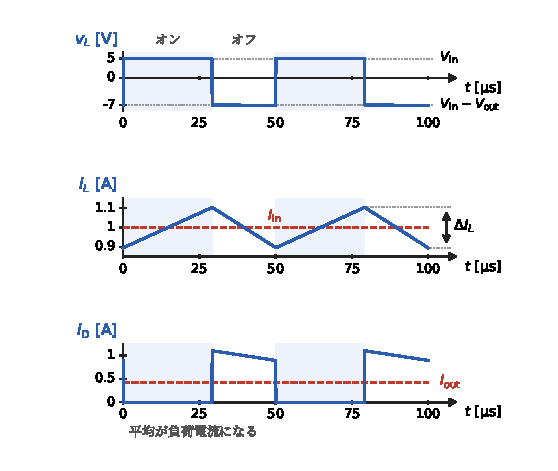
\includegraphics[clip]{figures/fig5.6.eps}
\end{center}
\caption{リプル電圧の発生。$i_C$が正の間（$T/2$の間），
斜線部の電荷$\mathit{\Delta}Q$がキャパシタに蓄えられ，電圧を$\mathit{\Delta}V_{\mathrm{out}}$だけ押し上げる。電圧の山と谷は$i_C$のゼロ交差の時刻に現れる}
\label{fig5.6}
\end{figure}

\subsection{リプル電圧を求める}

\FIGref{fig5.6}を見ながら，1周期の間の電圧の揺れ幅を求めよう。キャパシタの電圧は$i_C > 0$の間だけ上がり続ける。
$i_C$は平均ゼロの三角波だから，正である時間はちょうど半周期$T/2$である。
その間に流れ込む電荷$\mathit{\Delta}Q$は図の斜線部（三角形）の面積であり，底辺$T/2$，高さ$\mathit{\Delta}I_L/2$だから
\begin{equation}
\mathit{\Delta}Q = \frac{1}{2} \cdot \frac{T}{2} \cdot \frac{\mathit{\Delta}I_L}{2}= \frac{\mathit{\Delta}I_L\, T}{8}
\label{eq5.23}
\end{equation}
である。電荷$\mathit{\Delta}Q$の流入で電圧は$\mathit{\Delta}Q / C$だけ上がるから，リプル電圧は
\begin{equation}
\mathit{\Delta}V_{\mathrm{out}} = \frac{\mathit{\Delta}Q}{C}= \frac{\mathit{\Delta}I_L}{8 f C}
\label{eq5.24}
\end{equation}
となる。リプル電流と同じく，$C$を大きくするか$f$を高くすれば小さくできる。

\begin{screen}
\noindent\textbf{手順：リプル電圧からキャパシタを決める（降圧チョッパ）}\\[3pt]
\begin{enumerate}
\item 許容リプル電圧$\mathit{\Delta}V_{\mathrm{out}}$を決める（目安：$V_{\mathrm{out}}$の1\,\%程度）
\item \ref{sec5.5}節で決めた$\mathit{\Delta}I_L$を使い，式\ref{eq5.24}を$C$について解いて
\begin{equation}
C = \frac{\mathit{\Delta}I_L}{8 f\, \mathit{\Delta}V_{\mathrm{out}}}
\label{eq5.25}
\end{equation}
\item 選んだキャパシタの等価直列抵抗によるリプル（下の注意）を確かめる
\end{enumerate}
\end{screen}

\begin{例題}[キャパシタの設計]
\label{rei5.4}
例題\ref{rei5.3}の降圧チョッパ（$f = 100$\,kHz，$\mathit{\Delta}I_L = 0.4$\,A）で，
リプル電圧を$\mathit{\Delta}V_{\mathrm{out}} = 50$\,mV（出力$5$\,Vの1\,\%）に抑えたい。必要なキャパシタンスを求めよ。
\begin{解答}
式\ref{eq5.25}より
\begin{eqnarray}
C &=& \frac{\mathit{\Delta}I_L}{8 f\, \mathit{\Delta}V_{\mathrm{out}}}
= \frac{0.4}{8 \times 100 \times 10^{3} \times 0.05} \nonumber\\
&=& 10\,\mathrm{\mu F} \nonumber
\end{eqnarray}
リプル電流$0.4$\,Aに対してわずか$10\,\mathrm{\mu F}$で済むのは，スイッチング周波数が高いからである（\ref{sec5.8}節）。
\end{解答}
\end{例題}

\begin{注意}
実際のキャパシタには\index{とうかちょくれつていこう@等価直列抵抗}\textbf{等価直列抵抗}
（\index{いーえすあーる@ESR}ESR：equivalent series resistance。4章）$r_C$があり，リプル電流が流れるとそれだけで$r_C\, \mathit{\Delta}I_L$の電圧の揺れが生じる。
高いスイッチング周波数では式\ref{eq5.24}の項よりESRの項が支配的になることが多く，
電解キャパシタ（ESR大）よりセラミックキャパシタ（ESR小）が選ばれる理由になっている。式\ref{eq5.25}で求めた$C$は「最低限この容量」という下限と考えるのがよい。
\end{注意}

\begin{問}
\item 降圧チョッパで$V_{\mathrm{in}} = 10$\,V，$D = 0.5$，$f = 1$\,kHz，
$L = 30$\,mH，$C = 100\,\mathrm{\mu F}$のとき，リプル電流$\mathit{\Delta}I_L$とリプル電圧$\mathit{\Delta}V_{\mathrm{out}}$を求めよ
（この定数は章末問題\ref{ex5.6}のLTspice演習と同じである）。
\end{問}

%%======================================================================
\section{電流不連続モード}
\label{sec5.7}

\subsection{軽負荷で仮定が崩れる}

ここまで「インダクタ電流は常に正」と仮定してきた。この仮定が崩れるのはどんなときか。\ref{fig5.2}の$i_L$の谷の値は
\begin{equation}
i_{L,\min} = I_{\mathrm{out}} - \frac{\mathit{\Delta}I_L}{2}
\label{eq5.26}
\end{equation}
である。リプル電流$\mathit{\Delta}I_L$は式\ref{eq5.19}のとおり
負荷によらず一定だから，負荷電流$I_{\mathrm{out}}$が減っていくと（\index{けいふか@軽負荷}\textbf{軽負荷}），
やがて谷が0に触れ，さらに負荷が軽くなると電流が0に張り付く期間が現れる（\FIGref{fig5.7}）。
ダイオードは逆向きに電流を流せないので，電流が0に達した瞬間に勝手にオフしてしまうからである。

\begin{figure}[ht]
\begin{center}
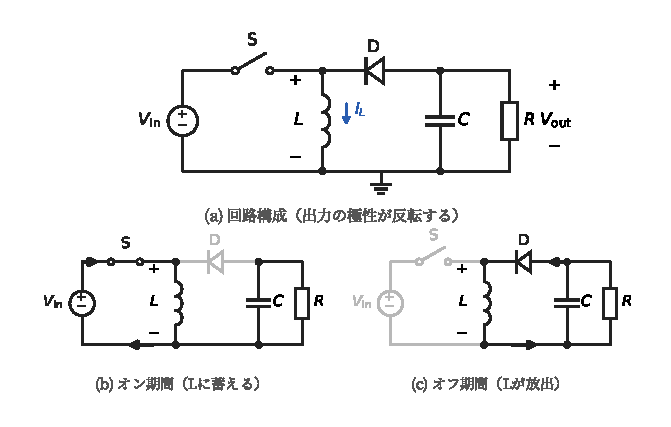
\includegraphics[clip]{figures/fig5.7.eps}
\end{center}
\caption{インダクタ電流のモード。負荷電流が$\mathit{\Delta}I_L/2$を下回ると，電流が0に張り付く第3の期間が現れる（DCM）}
\label{fig5.7}
\end{figure}

\begin{定義}[電流連続モードと電流不連続モード]
\label{def5.2}
インダクタ電流が1周期を通して正であるとき\textbf{電流連続モード}（\index{しーしーえむ@CCM}CCM：continuous conduction mode），
電流が0に張り付く期間があるとき\index{でんりゅうふれんぞくもーど@電流不連続モード}\textbf{電流不連続モード}
（\index{でぃーしーえむ@DCM}DCM：discontinuous conduction mode）という。その境目は，谷がちょうど0に触れる
\begin{equation}
I_{\mathrm{out}} = \frac{\mathit{\Delta}I_L}{2}= \frac{(V_{\mathrm{in}} - V_{\mathrm{out}})\, D}{2 f L}
\label{eq5.27}
\end{equation}
のときである（降圧チョッパの場合）。
\end{定義}

\subsection{DCMでは電圧比が$D$だけで決まらない}

DCMに入ると何が変わるか。1周期が「オン」「オフ（電流あり）」に加えて，
\textbf{Sも$\mathrm{D}$も導通せず$i_L = 0$のまま止まっている第3の期間}をもつようになる（\ref{fig5.7}(c)）。この期間は$v_L = 0$だから，ボルト秒平衡の式\ref{eq5.5}は
\begin{equation*}
V_{\mathrm{on}} \cdot DT + V_{\mathrm{off}} \cdot D_2 T = 0
\end{equation*}
という形に変わる。ここで$D_2 T$は電流が減少している期間の長さで，$D_2$は負荷電流と$L$と$f$に依存して決まる（$D_2 < 1-D$）。
その結果，\textbf{出力電圧はもはや$D$だけでは決まらず}，負荷電流が軽いほど，また$L$が小さいほど，出力は式\ref{eq5.9}の値$D V_{\mathrm{in}}$より高く浮き上がる。
直感的には，軽い負荷が受け取りきれないエネルギーが毎周期送り込まれて，$C$の電圧が押し上げられるのである
（$V_{\mathrm{out}}$が上がると送り込まれるエネルギーが減るため，新しい釣合い点には落ち着く）。

一定の$D$で運転している電源の負荷が軽くなった途端に出力電圧が跳ね上がるのは困る。そこで実際の電源では，出力電圧を測って$D$を自動調整する
（フィードバック制御）か，DCMそのものを避ける対策を取る。DCMを避けるには次のいずれかが使われる。

\begin{箇条書}
\item 式\ref{eq5.27}より，$L$を大きくするか$f$を高くして$\mathit{\Delta}I_L$自体を小さくする
\item ダイオードをスイッチ（MOSFET）に置き換えて逆向きの電流も流せるようにする
（\index{どうきせいりゅう@同期整流}\textbf{同期整流}。電流は0を横切って負にもなれるので，どんな軽負荷でもCCMを保てる。
ダイオードの順方向電圧降下がなくなるため効率も上がる）
\end{箇条書}

\begin{問}
\item 例題\ref{rei5.3}の設計（$12$\,V→$5$\,V，$f = 100$\,kHz，
$L = 73\,\mathrm{\mu H}$，$\mathit{\Delta}I_L = 0.4$\,A）で，負荷電流がいくら以下になるとDCMに入るか。またそのときの負荷抵抗はいくら以上か。
\end{問}

%%======================================================================
\section{高周波化による小型化}
\label{sec5.8}

本章の設計式をあらためて眺めると，重要なことに気づく。
必要なインダクタンス（式\ref{eq5.21}）もキャパシタンス（式\ref{eq5.25}）も，分母にスイッチング周波数$f$をもつ ―
つまり\textbf{同じリプルを許すなら，$f$を10倍にすれば$L$も$C$も10分の1で済む}（\FIGref{fig5.8}）。インダクタとキャパシタは電源の体積の大半を占める部品だから，
\index{こうしゅうはか@高周波化}\textbf{高周波化}はそのまま電源の小型化・軽量化につながる。単位体積あたりに変換できる電力
（\index{ぱわーみつど@パワー密度}\textbf{パワー密度}）を高める最も効く手段である。

\begin{figure}[ht]
\begin{center}
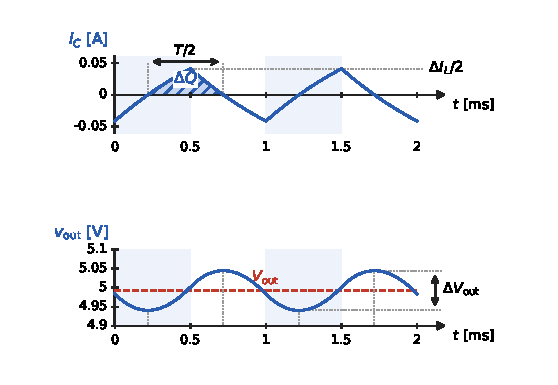
\includegraphics[clip]{figures/fig5.8.eps}
\end{center}
\caption{スイッチング周波数と必要な$L$・$C$（例題\ref{rei5.3}・例題\ref{rei5.4}の設計仕様の場合）。リプルを一定に保つなら，どちらも$1/f$で小さくできる}
\label{fig5.8}
\end{figure}

ただし高周波化はただでは手に入らない。スイッチの切替え1回ごとに失われるエネルギーはほぼ決まっているから，
\index{すいっちんぐそんしつ@スイッチング損失}\textbf{スイッチング損失}は$f$に比例して増える（3章）。
インダクタの磁性材料の損失も周波数とともに増える。発熱が許す範囲でどこまで$f$を上げられるかは，
スイッチング速度に優れたデバイス ― まさに3章で学んだSiC・GaNの得意分野 ― で決まる。
さらに，急峻な電圧・電流の切替えは電磁ノイズの発生源でもあり，高周波化はノイズ対策（EMC）との戦いでもある。これは11章で正面から扱う。

こうして本章の3回路は，「エネルギーを$L$に蓄えて放出する比率で電圧を作り替える」という1つの原理と，
「リプルから$L$と$C$を決める」という1つの設計手順で貫かれていることがわかった。ただし非絶縁型には，入力と出力が電気的につながったままという弱点がある。
感電の防止や大きな電圧比のためには入出力を切り離したい ― その要求に応えるのが，次章の絶縁型DC-DCコンバータである。

%%======================================================================
\begin{章末問題}
\item \label{ex5.1}入力$24$\,Vから$12$\,V・$3$\,Aを作る降圧チョッパを設計する。スイッチング周波数は$f = 200$\,kHzとする。
\begin{enumerate}
\item[(a)] デューティ比$D$を求めよ。
\item[(b)] リプル電流を$0.6$\,A（負荷電流の2割）に抑えるための$L$を求めよ。
\item[(c)] リプル電圧を$50$\,mVに抑えるための$C$を求めよ。
\item[(d)] インダクタ電流の最大値を求めよ。
\end{enumerate}

\item \label{ex5.2}バッテリー$12$\,Vから$48$\,V・$0.5$\,Aを作る昇圧チョッパ（$f = 100$\,kHz，$L = 100\,\mathrm{\mu H}$）について，損失を無視して答えよ。
\begin{enumerate}
\item[(a)] デューティ比$D$と入力電流$I_{\mathrm{in}}$を求めよ。
\item[(b)] リプル電流$\mathit{\Delta}I_L$とインダクタ電流の最大値を求めよ。オン期間の$v_L = V_{\mathrm{in}}$から計算すればよい。
\item[(c)] オフ期間にスイッチSが受け持つ電圧と，オン期間にダイオードが受け持つ電圧を求めよ。素子の耐圧は入力と出力のどちらの電圧で決まるか。
\end{enumerate}

\item \label{ex5.3}昇降圧チョッパについて，オン期間とオフ期間の等価回路を描き，ボルト秒平衡から式\ref{eq5.18}を導け。
また，入力$12$\,Vから大きさ$12$\,V，$5$\,V，$24$\,Vの負電圧を得るためのデューティ比をそれぞれ求めよ。

\item \label{ex5.4}降圧チョッパがCCMを保つ条件を負荷抵抗$R$で表そう。
\begin{enumerate}
\item[(a)] $I_{\mathrm{out}} = V_{\mathrm{out}}/R$と式\ref{eq5.27}から，CCMとDCMの境界の負荷抵抗が$R_B = \dfrac{2 f L}{1-D}$と書けることを示せ。
\item[(b)] 例題\ref{rei5.3}の設計（$D = 0.417$，$f = 100$\,kHz，$L = 73\,\mathrm{\mu H}$）の$R_B$を求め，\ref{sec5.7}節の問の結果と一致することを確かめよ。
\end{enumerate}

\item \label{ex5.5}ダイオードの順方向電圧降下$V_F$を無視しない場合の降圧チョッパを考える（それ以外の仮定はそのまま）。
\begin{enumerate}
\item[(a)] オフ期間のインダクタ電圧が$v_L = -V_{\mathrm{out}} - V_F$となることを示し，ボルト秒平衡から$V_{\mathrm{out}} = D V_{\mathrm{in}} - (1-D) V_F$を導け。
\item[(b)] $V_{\mathrm{in}} = 12$\,V，$D = 0.417$，$V_F = 0.7$\,Vのとき
出力電圧はいくらか。理想値$5$\,Vからのずれを求めよ。この損失を避けるために\ref{sec5.7}節の同期整流が使われる。
\end{enumerate}

\item \label{ex5.6}
（LTspiceで確かめよ）配布モデル\texttt{LTspice/Lecture5/back\_withC}の降圧チョッパ（$V_{\mathrm{in}} = 10$\,V，$D = 0.5$，$f = 1$\,kHz，$L = 30$\,mH，
$C = 100\,\mathrm{\mu F}$，$R = 10\,\Omega$）をシミュレーションし，次を確かめよ。
\begin{enumerate}
\item[(a)] 定常状態の$\mathit{\Delta}I_L$と$\mathit{\Delta}V_{\mathrm{out}}$を
波形から読み取り，式\ref{eq5.19}・式\ref{eq5.24}の計算値（\ref{sec5.6}節の問）と比較せよ。
\item[(b)] 負荷を$R = 150\,\Omega$に変えると波形はどう変わるか。
出力電圧が$5$\,Vより高くなることを確かめ，理由を説明せよ（境界は章末問題\ref{ex5.4}の$R_B$で見積もれる）。
\item[(c)] $f$を$10$\,kHzに上げると，$R = 10\,\Omega$のままで$\mathit{\Delta}I_L$と$\mathit{\Delta}V_{\mathrm{out}}$はどうなるか。式から予想してから確かめよ。
\item[(d)] $L$を$3$\,mHに減らすと$\mathit{\Delta}I_L$はどうなるか。また$R = 150\,\Omega$のままではモードはどうなるか。予想してから確かめよ。
\end{enumerate}
\end{章末問題}
